\usepackage[utf8]{inputenc}
\usepackage{tikz}
\usetikzlibrary{chains,fit,shapes}
\usepackage[export]{adjustbox}

\usepackage[americaninductors]{circuitikz}
 \usetikzlibrary{arrows}
\usepackage[T1]{fontenc}
\usepackage[nolist,nohyperlinks]{acronym} 
\acrodef{CMU}[CMU]{Clock Monitoring Unit}
\acrodef{DPA}[DPA]{Differential Power Analysis}
\acrodef{FCT}[FCT]{Funda\c{c}\~ao para a Ci\^encia e Tecnologia}
\acrodef{fdsoi}[FD-SOI]{Fully-Depleted Silicon-On-Insulator}
\acrodef{ff}[FF]{flip-flop}
\acrodef{FFT}[FFT]{Fast Fourier Transform}
\acrodef{FLL}[FLL]{frequency-locked loop}
\acrodef{GPS}[GPS]{Global Positioning System}
\acrodef{HD}[HD]{Hamming distance}
\acrodef{IC}[IC]{Integrated Circuit}
\acrodef{INESC-ID}[INESC-ID]{Instituto de Engenharia e Sistemas}
\acrodef{LCD}[LCD]{liquid-crystal display}
\acrodef{LDPC}[LDPC]{Low-density Parity-check}
\acrodef{MOM}[MOM]{metal-oxide-metal}
\acrodef{OTA}[OTA]{Operational Transconductance Amplifier}
\acrodef{OTP}[OTP]{one-time password}
\acrodef{pdf}[pdf]{probability density function}
\acrodef{PLL}[PLL]{Phase-Locked Loop}
\acrodefplural{PRNG}[PRNGs]{Pseudorandom Number Generators}
\acrodefplural{PUF}[PUFs]{Physically Unclonable Functions }
\acrodefplural{PUF}[PUFs]{Physically Unclonable Functions}
\acrodefplural{RO}[ROs]{Ring Oscillators}
\acrodefplural{TRNG}[TRNGs]{True Random Number Generators}
\acrodef{pmf}[pmf]{probability mass function}
\acrodef{PRNG}[PRNG]{Pseudorandom Number Generator}
\acrodef{PUF}[PUF]{Physically Unclonable Function }
\acrodef{PUF}[PUF]{Physically Unclonable Function}
\acrodef{PVT}[PVT]{Process, Voltage and Temperature}
\acrodef{RC}[RC]{Resistor and Capacitor}
\acrodef{RF}[RF]{Radio-Frequency}
\acrodef{RO}[RO]{Ring Oscillator}
\acrodef{RTC}[RTC]{real-time clock}
\acrodef{SNR}[SNR]{Signal-to-Noise Ratio}
\acrodef{SoC}[SoC]{System on a Chip}
\acrodef{SoCs}[SoCs]{Systems on a Chip}
\acrodef{TERO}[TERO]{Transient-Effect Ring Oscillator}
\acrodef{TRNG}[TRNG]{True Random Number Generator}
\acrodef{TM}[TM]{Turing Machine}


\usepackage{siunitx}                              
\newsavebox{\amplimiter}
\savebox{\amplimiter}{%
    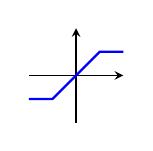
\begin{tikzpicture}[font=\small,
            >=stealth,
        ]
        \draw[->,black] (-0.6,0) -- (0.6,0);
        \draw[->,black] (0,-0.6) -- (0,0.6);
        \draw[thick,blue] (-0.6,-0.3) -- (-0.3,-0.3) -- (0.3,0.3) -- (0.6,0.3) ;
       % \draw[thick, blue] (0,0) --(0.2,0) ..controls (0.5,1)..(1,1)..controls(1.2,1) and (1.8,0)..  
       %     node[black,left]{$H(f)$} (2,0) -- (2.5,0);
       % \draw (0,0) node[below]{$0$} (1,0) node[below]{$f$} (2,0) node[below]{$\rightarrow\infty$};
    \end{tikzpicture}%
}

\newsavebox{\softinv}
\savebox{\softinv}{%
    
\begin{tikzpicture}[font=\small,
            >=stealth,
        ]
        %\draw[->,black] (-0.6,0) -- (0.6,0);
        %\draw[->,black] (0,-0.6) -- (0,0.6);
        \draw[thick,blue] (-0.6,-0.3) -- (-0.3,-0.3) -- (0.3,0.3) -- (0.6,0.3) ;
        \draw[thick,blue] (-0.6,0.3) -- (-0.3,0.3) -- (0.3,-0.3) -- (0.6,-0.3) ;
       % \draw[thick, blue] (0,0) --(0.2,0) ..controls (0.5,1)..(1,1)..controls(1.2,1) and (1.8,0)..  
       %     node[black,left]{$H(f)$} (2,0) -- (2.5,0);
       % \draw (0,0) node[below]{$0$} (1,0) node[below]{$f$} (2,0) node[below]{$\rightarrow\infty$};
    \end{tikzpicture}%
}


\usepackage{color}
\sisetup{detect-weight=true, detect-family=true}
              


\mode<presentation> {

\usetheme{Lisbon}
%\setbeamertemplate{footline} % To remove the footer line in all slides uncomment this line
%\setbeamertemplate{footline}[page number] % To replace the footer line in all slides with a simple slide count uncomment this line

%\setbeamertemplate{navigation symbols}{} % To remove the navigation symbols from the bottom of all slides uncomment this line
}

\usepackage{graphicx} % Allows including images
\usepackage{booktabs} % Allows the use of \toprule, \midrule and \bottomrule in tables

%----------------------------------------------------------------------------------------
%	TITLE PAGE
%----------------------------------------------------------------------------------------

\title[DPInfSec - 1\textsuperscript{st} year]{Doctoral Programme in Information Security} 
\subtitle{ 1\textsuperscript{st} year -  Coursework} 
\institute[IST] 
{
%Coursework \\
%\medskip
Instituto Superior T\'{e}cnico, Universidade de Lisboa \\ 
\medskip
\textit{jose.leitao@tecnico.ulisboa.pt} 
}
\author{Jos\'{e} M. Leit\~{a}o }
\date 

\begin{document}

\begin{frame}[plain]
\titlepage % Print the title page as the first slide
\end{frame}

\begin{frame}
\frametitle{Overview} % Table of contents slide, comment this block out to remove it
\tableofcontents % Throughout your presentation, if you choose to use \section{} and \subsection{} commands, these will automatically be printed on this slide as an overview of your presentation
\end{frame}

\section[Theory. of Computability \& Complexity]{Theory of Computatibility, Complexity and Information}
\begin{frame}
\frametitle{Mathematical Model of Computation}


\begin{block}
{Turing Machine (TM)}
Abstract machine (computer) able to sequentially read/write symbols on an infinite tape by shifting its \emph{head} right or left.
\end{block}
\begin{figure}
\center
%!TEX root = Notes.tex
%\newcommand{\tape[1][]{% 1 optional parameter for options for the tikz picture
%\begin{tikzpicture}[#1]
\begin{tikzpicture}
\tikzstyle{every path}=[very thick]

\edef\sizetape{0.7cm}
\tikzstyle{tmtape}=[draw,minimum size=\sizetape]
\tikzstyle{tmhead}=[arrow box,draw,minimum size=.5cm,arrow box
arrows={east:.25cm, west:0.25cm}]
%% Draw TM tape
\begin{scope}[start chain=1 going right,node distance=-0.15mm]
    %\node [on chain=1,tmtape,draw=none] {$\ldots$};
    \node [on chain=1,tmtape] (input) {$w_1$};
    \node [on chain=1,tmtape] {B};
    \node [on chain=1,tmtape] {$w_2$};
    \node [on chain=1,tmtape] {B};
    \node [on chain=1,tmtape] {$\ldots$};
    \node [on chain=1,tmtape] {$w_n$};
    \node [on chain=1,tmtape] {B};
    \node [on chain=1,tmtape] {$\ldots$};
     \node [on chain=1,tmtape] {B};
    %\node [on chain=1,tmtape,draw=none] {$\ldots$};
   % \node [on chain=1] {\textbf{Input/Output Tape}};
\end{scope}
%% Draw TM head below (input) tape cell
\node [tmhead,yshift=-.3cm] at (input.south) (head) {\tiny \bf head };
\end{tikzpicture}
%} 

\end{figure}

\pause
A function $\phi :\mathbb{N} \rightarrow \mathbb{N} $ is said to be a {\bf partial computable} function if there exists a Turing Machine $M$ such that
\begin{align*}
f_M =\phi 
\end{align*}

\pause
A Turing Machine $M$ admits an encoding in  $\mathbb{N}$ (or in $\{0,1\}^\star$).


\note<1>{%\subsection{}
%\subsection*{Turing Machine}
A Turing Machine $M(Q,\Sigma,\Gamma,\delta,q_0,q_a,q_r,B)$ is a set where:
\begin{itemize} 
\item $Q$ is a finite set of states 
\item $\Gamma$ is a finite set of symbols called the \textbf{tape alphabet }
\item $ B \in \Gamma$  is the blank symbol
\item $ \Sigma \subseteq \Gamma \setminus\{B\}$ is the \textbf{input alphabet}
\item $ \delta : Q \setminus\{q_a,q_h\}\times \Gamma \rightarrow Q\times\Gamma\times \{L,R\}$ is the \textbf{transition function}
\item $q_0 \in Q $ is the initial state
\item $q_a \in Q $ is the accept state
\item $q_r \in Q $ is the reject state
\end{itemize}

\begin{figure}

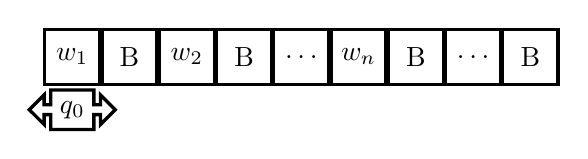
\begin{tikzpicture}
\tikzstyle{every path}=[very thick]

\edef\sizetape{0.7cm}
\tikzstyle{tmtape}=[draw,minimum size=\sizetape]
\tikzstyle{tmhead}=[arrow box,draw,minimum size=.5cm,arrow box
arrows={east:.25cm, west:0.25cm}]
%% Draw TM tape
\begin{scope}[start chain=1 going right,node distance=-0.15mm]
    %\node [on chain=1,tmtape,draw=none] {$\ldots$};
    \node [on chain=1,tmtape] (input) {$w_1$};
    \node [on chain=1,tmtape] {B};
    \node [on chain=1,tmtape] {$w_2$};
    \node [on chain=1,tmtape] {B};
    \node [on chain=1,tmtape] {$\ldots$};
    \node [on chain=1,tmtape] {$w_n$};
    \node [on chain=1,tmtape] {B};
    \node [on chain=1,tmtape] {$\ldots$};
     \node [on chain=1,tmtape] {B};
    %\node [on chain=1,tmtape,draw=none] {$\ldots$};
   % \node [on chain=1] {\textbf{Input/Output Tape}};
\end{scope}
%% Draw TM head below (input) tape cell
\node [tmhead,yshift=-.3cm] at (input.south) (head) {$q_0$};
\end{tikzpicture}
\end{figure}
%
%A Turing Machine computes a (partial) function $f_M: (\Sigma^\star)^n \rightarrow \Sigma^\star $ when, at the initial state, the tape is 

 %%!TEX root = Notes.tex
%\newcommand{\tape[1][]{% 1 optional parameter for options for the tikz picture
%\begin{tikzpicture}[#1]
\begin{tikzpicture}
\tikzstyle{every path}=[very thick]

\edef\sizetape{0.7cm}
\tikzstyle{tmtape}=[draw,minimum size=\sizetape]
\tikzstyle{tmhead}=[arrow box,draw,minimum size=.5cm,arrow box
arrows={east:.25cm, west:0.25cm}]
%% Draw TM tape
\begin{scope}[start chain=1 going right,node distance=-0.15mm]
    %\node [on chain=1,tmtape,draw=none] {$\ldots$};
    \node [on chain=1,tmtape] (input) {$w_1$};
    \node [on chain=1,tmtape] {B};
    \node [on chain=1,tmtape] {$w_2$};
    \node [on chain=1,tmtape] {B};
    \node [on chain=1,tmtape] {$\ldots$};
    \node [on chain=1,tmtape] {$w_n$};
    \node [on chain=1,tmtape] {B};
    \node [on chain=1,tmtape] {$\ldots$};
     \node [on chain=1,tmtape] {B};
    %\node [on chain=1,tmtape,draw=none] {$\ldots$};
   % \node [on chain=1] {\textbf{Input/Output Tape}};
\end{scope}
%% Draw TM head below (input) tape cell
\node [tmhead,yshift=-.3cm] at (input.south) (head) {\tiny \bf head };
\end{tikzpicture}
%} 
 
 %whenever $\{w_1,w_2,\ldots,w_n\} \in \text{Dom}(f)$


}
\note<2>{There are  $\mathbb{N}^\mathbb{N}$ functions from   $\{0,1\}^\star\to \{0,1\}^\star$ 
but only $\mathbb{N}$ (\emph{countably} many) computable functions (or programs)
so there are many more (\emph{uncountably} many) functions that are not computable!
}
\note<3>{{\bf Total Function}

A function  $\phi$ is said to be a {\bf total computable function} if 

\begin{align} 
\phi \text{ is partial computable and } \text{Dom}(\phi) =  (\Sigma^\star)^n
\end{align}

{\bf Decidable Set}

A  set $S$ is said to be decidable if there is a Turing Machine $M$ such that:

\begin{align} 
   \begin{cases}
 s \in  S \implies M  \text{ accepts } \\    
  s \notin  S  \implies M  \text{ rejects }   
\end{cases}
\end{align}
{\bf Proposition:}    $S $ is decidable $\iff  X_S $ is totally computable 
\begin{align} 
   X_S(s) =  \begin{cases}
1 \text{ if } s \in S \\
0 \text{ otherwise} \\
\end{cases}
\end{align}
 
}
\end{frame}


\begin{frame}
\frametitle{Complexity and Information Theory}
{\scriptsize Classifying the \emph{hardness} of a problem:}
\begin{block}
{Time Complexity}
The number of elementary steps (r/w + head shifts) required to run an algorithm that solves the problem.
\end{block}

\pause
{\scriptsize Quantifiying the \emph{randomness} of a string:}
\begin{block}
{Kolmogorov Complexity}
The complexity of a string as the length of the shortest computer program that outputs the string.
\end{block}
\pause
{\scriptsize Measuring the \emph{amount of information} in (knowing) a physical state:} 
\begin{block}
{Information Entropy}
\begin{align*}
-\sum_X  p(x)\log{p(x)}
\end{align*}
\end{block}

\note{Example:
$P\neq NP ?$

\begin{align*}
10101010101010101010101010101010101010101010101010\\
00011101001000101101001000101111010100000100111101
\end{align*}
Yet, by the immutable laws of probability, each string has an equal chance ($2^{-50}$) in being chosen at random from all sequences of 50 binary digit


}
\end{frame}


\section[Physics of Information]{Physics of Classical and Quantum Information}

\begin{frame}
\frametitle{Physics of Information}
\begin{block}{Landauer's bound [1961]}
Any {\bf irreversible} logical operation cannot dissipate less than
\begin{align*}
E_{min} &=k_B T \log 2  
\end{align*}
\note{   Two-state physical system set/reset operation:
    \begin{itemize}
    \item Initial state: $S^i_S=k_B \log2$
    \item Final state: $S^f_S=-k_B \log2$
    \end{itemize}
    \begin{align*}
    \Delta S_T &= \Delta S_S + \Delta S_E \ge 0 \\
    \Delta S_E &\geq - \Delta S_S \\ 
    \Delta S_E &\geq k_B\log 2\\
    \Delta Q_E &= T \Delta S_E \geq k_B T \log 2 \\
    \end{align*}
    
}
\end{block}

\begin{itemize}
\item  T= 300 K $\implies E_{min} \approx  3 \times 10^{-21} \si{\joule}$
\end{itemize}

\pause
\underline{\href{file:../../../courses/PCQI/presentation/main.pdf}{CMOS technology is still far from this limit} }
\pause

\vspace{1em}
\emph{Example:} 1-bit NOT gate C=\SI{1}{\femto\farad} and V=\SI{1}{\volt}
\begin{align*}
E_{diss} \approx CV^2 &\approx  10^{-15} \si{\joule} \approx {\color{blue} 10^6} \times E_{min}
\end{align*}
\end{frame}


\begin{frame}
\frametitle{Quantum Computing}
\begin{minipage}{0.6\columnwidth}
Carrying information  in  quantum states $\iff$ {\bf qu}bits
lead to a new computing paradigm, leveraging \emph{entanglement}.
\end{minipage}
\begin{minipage}{0.3\columnwidth}
\hfill \includegraphics[scale=0.35]{img/Bloch_sphere.png}
\end{minipage}

\pause

\begin{block}
{Schor's Algorithm}
Solves prime factorization in {\bf P} by 
translating it into a phase estimation algorithm (Quantum FFT).
\end{block}
\pause
Breaks most classical (public-key) cryptosystems (RSA,DH,ECC,...), hence the need for:
\begin{itemize}
\item Quantum Cryptography
\item  \href{https://csrc.nist.gov/Projects/Post-Quantum-Cryptography/Round-1-Submissions}{Post-quantum Cryptography}  
\end{itemize}

\end{frame}

\section[Cryptography]{Cryptography and Security Protocols}

\begin{frame}
\frametitle{Cryptographic system}

A cryptosystem is a tuple $\mathcal{(X,Y,K,E,D)}$ where:
\begin{align*}
\mathcal{X} &\text{ is a finite set of} \textit{ plaintexts}\\
\mathcal{Y}&\text{ is a finite set of} \textit{ ciphertexts}\\
\mathcal{K}&\text{ is a finite set of} \textit{ keys}\\
\mathcal{E}&=\{e_k:\mathcal{X}\to \mathcal{Y} \}_{k \in \mathcal{K} } \text{ is a family of} \textit{ encryption maps}\\
\mathcal{D}&=\{d_k:\mathcal{Y}\to \mathcal{X} \}_{k \in \mathcal{K} } \text{ is a family of} \textit{ decryption maps}\\
\end{align*}
{\bf such that:}
$ d_k(e_k(x))=x, \forall_k \in K$
\begin{block}
{Shannon's Theorem }
A cryptosystem is said to be perfectly secure if
\begin{align*}
P(X=x|Y=y)&=P(X=x)
\end{align*}
\end{block}
\end{frame}

\begin{frame}
\frametitle{Cryptographic Systems - Math Background }
\begin{itemize}
\item Symmetric Cryptosystems - OTP, DES, AES  
\begin{itemize}
\item S-BOX
\end{itemize}
\item Asymmetric Cryptosystems - DH, RSA, ECC, ElGamal
\begin{itemize}
\item Signature schemes
\end{itemize}
\item Hash Functions
\begin{itemize}
\item Strong collision-free
\item Weak collision-free
\end{itemize}
\item Secret-sharing
\item Zero-knowledge
\item Bit commitment
\item Yao's garbled circuits
\begin{itemize}
\item Millionaire dilemma : $f(x_1 , x_2 ) =  \chi_{x_1 < x_2} (x_1 , x_2 )$  
\end{itemize}

\end{itemize}
\note{\begin{itemize}
\item Strong collision-free
    \begin{itemize}
    \item Hard to find matching pair $x,x'$ s.t. $h(x)=h(x')$
    \end{itemize}
\item Weak collision-free
    \begin{itemize}
    \item Given $x$, hard to find $x'$ s.t. $h(x)=h(x')$
    \end{itemize}
\end{itemize}
}
\end{frame}

\section[Statistical Learning]{Statistical Learning}

\begin{frame}
\frametitle{Decision Theory}
\begin{itemize}
\item Bayesian Decision Theory
\begin{align*}
f_{S|X}(s|x)= \frac{f_{X|S}(x|s) f_S(s)}{f_X(x)} = \frac{\text{"likelihood"}\times\text{"prior"}}{\text{"evidence"}} = \text{"posterior"}
\end{align*}

\item Linear Regression
\begin{itemize}
\item Estimate $f_{XY}(x,y)$  - \emph{Generative Perspective}
\item Estimate $f_{X|Y}(x|y)$  - \emph{Discriminative Perspective}
\end{itemize}
\item Ridge Regression (Regularization)
\item Support Vector Machines (Classification)
\item Probabilistic Graphical Models
\begin{align*}
\end{align*}
\end{itemize}
\end{frame}

\begin{frame}
\frametitle{Statistical Inference in the Analog Domain}
\begin{minipage}{0.4\columnwidth}
\begin{itemize}
\item Factor Graphs
\begin{itemize}
\item Belief Propagation
\end{itemize}
\vspace{1em}
\item Analog Computing
\begin{itemize}
\item LDPC decoding  
\item LFSR sync
\item \emph{Soft-gates}
\end{itemize}
\end{itemize}
\vspace{1em}
\scalebox{1}{ \begin{circuitikz}[]
    \draw
        (0,0) node[not port] (stage1) {} 
        ;
    
       \draw (stage1.in) --++(-1,0)node[midway,anchor=south]{$x$};
       \draw (stage1.out) --++(1,0)node[midway,anchor=south]{$y$};
\end{circuitikz}
}
\small
\begin{align*}
p_{z}&=1-p_X(z)
\end{align*}
%\vspace{2em}
\end{minipage}
\hfill
\begin{minipage}{0.5\columnwidth}
\centering \scalebox{0.8}{ 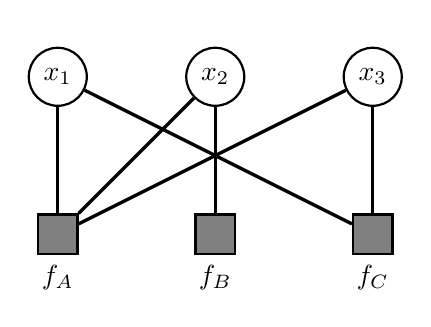
\begin{tikzpicture}[
every edge/.style = {draw=black,very thick},
 vrtx/.style args = {#1/#2}{%
      circle, draw, thick, fill=white,
      minimum size=5mm, label=#1:#2},
 factor/.style args = {#1/#2}{%
      rectangle, draw, thick, fill=gray,
      minimum size=5mm, label=#1:#2}
                    ]
\node(x1) [vrtx=/] at (0, 1) {$x_1$};
\node(fA) [factor=south/$f_A$] at (0,-1) {};
\node(x2) [vrtx=/] at (2, 1) {$x_2$};
\node(fB) [factor=south/$f_B$] at (2,-1) {};
\node(x3) [vrtx=/] at (4, 1) {$x_3$};
\node(fC) [factor=south/$f_C$] at (4,-1) {};
%
\path   (x1)  edge (fA);
\path   (x2)  edge (fB);
\path   (x1)  edge (fC);
\path   (x3)  edge (fC);
\path   (x3)  edge (fA);
\path   (x2)  edge (fA);
\end{tikzpicture}
}
\small
\begin{align*}
p(x_1,x_2,x_3)=f_A(x_1,x_2,x_3) f_B(x_2)f_C(x_1,x_3)
\end{align*}
\scalebox{1}{ 
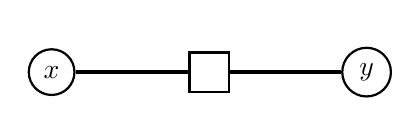
\begin{tikzpicture}[
every edge/.style = {draw=black,very thick},
 vrtx/.style args = {#1/#2}{%
      circle, draw, thick, fill=white,
      minimum size=5mm, label=#1:#2},
 factor/.style args = {#1/#2}{%
      rectangle, draw, thick, fill=white,
      minimum size=5mm, label=#1:#2}
                    ]
\node(x) [vrtx=/] at (0, 0) {$x$};
\node(inv) [factor=/] at (2, 0) {\usebox{\softinv}};
\node(y) [vrtx=/] at (4, 0) {$y$};
%
\path   (x)  edge (inv);
\path   (inv)  edge (y);
\end{tikzpicture}
}
\small
\begin{align*}
p_{X,Y}(x,y)&=p_X(x)\underbrace{\delta(x\oplus y = 1)}_{\text{constraint}}
\end{align*}
\end{minipage}

\end{frame}

\begin{frame}

{\Huge{\centerline{Thank you}}}
\vspace{2em}
{\small I would also like to acknowledge the support of everyone}

\end{frame}



